\section{目的}
依據 \textit{AIC Lab.pdf} PDF 41--47 頁，完整涵蓋 Lab 4.A 電壓差動放大器與 Lab 4.B 電流差動放大器。使用由使用者另行提供的模型庫，供應電壓為 1.0 V。這是本次教學適配條件，並非模型額定電壓的認證；講義原製程的 3.3 V 圖表與數字不直接當作通過門檻。程式依講義拓樸重寫，原始程式僅作尺寸與缺漏的參考。

\section{Spec 對照}
S 為實際模擬，D 為推導／討論。表中 D01 等為 netlist 的數字前綴；案例從 C0 開始。
\small\begin{longtable}{p{.46\linewidth}p{.30\linewidth}p{.15\linewidth}}\toprule
要求與 PDF 頁碼 & 對應 deck／檢查 & 狀態 \\ \midrule\endhead
三種差動電壓放大器（41--42） & D01--03 & S+D \\
ICMR 與各元件飽和檢查（42） & D04; 21 points & S+D \\
增益、GB、CMRR、PSRR（43--44） & D01--03; AC families & S+D \\
等 W/L 尺度與 cascode 比較（44） & D01/C4--6; D02--03 & S+D \\
三種電流放大器及 1 kOhm 負載（45--47） & D05 & S+D \\
100/1000/10000 um 尺寸與 Rin/Rout（46--47） & D05/C1--12 & S+D \\
PMOS 電流源尺寸及優缺點（47） & D05/C13 & S+D \\
\bottomrule\end{longtable}\normalsize


\section{電路與設計推導}
\[
 A_d\simeq\frac{g_m}{g_{ds,n}+g_{ds,p}},\qquad
 f_u\simeq\frac{g_m}{2\pi C_L},\qquad
 \mathrm{CMRR}_{dB}=20\log_{10}\left|\frac{A_d}{A_{cm}}\right|.
 \]
 \[
 \mathrm{PSRR}_{\pm,dB}=20\log_{10}\left|\frac{A_d}{A_{supply,\pm}}\right|,
 \quad R_{in}\simeq1/g_{m,in},\quad A_i\simeq\frac{(W/L)_{out}}{(W/L)_{in}}.
 \]電壓放大器的 $C_L=10$ pF；基本型參考電流 50 $\mu$A，cascode 基本比較另列為 0.5 $\mu$A，以保留 1 V 的電壓裕量，並保留原 50 $\mu$A 案例。M1/M2 為 $425/0.3\,\mu$m，PMOS 負載為 $1350/0.3\,\mu$m，參考／尾電流元件為 $85/0.3$ 與 $870/0.3\,\mu$m。D01/C4、C5 把輸入與負載的 W、L 同乘 3、5；尾電流鏡不變。全 cascode 的額外 NMOS 閘極固定 0.6 V。

電流放大器同時建立簡單型 s、cascode 型 c、差動型 d。參考 NMOS 寬 50 $\mu$m，輸出寬 100/1000/10000 $\mu$m，$L=0.3\,\mu$m，輸出接真實 1 k$\Omega$ 到地。C0 保留匹配來源與吸收電流，輸出偏壓可能接近地而失去工作區；C1--3 明列增加 PMOS 的名義 0.5 mA 偏流，使負載約落在 0.5 V。C7--9 改 cascode 下層兩管的寬度，C13 把 s/c 的 PMOS 電流源寬度加倍；d 的第一 PMOS 亦變，後兩顆依其固定比例，所以它是額外不平衡反例而非公平比較。

\section{模擬設定}
使用 PrimeSim HSPICE S-2021.09 win64，基本溫度 27 $^\circ$C，\texttt{runlvl=5}、\texttt{accurate}，輸出 \texttt{.op/.print/.measure}。每個 \texttt{.alter} 先重設完整基準參數與溫度，防止前一案例殘留。實際工作已完成，未出現 error 或 failed 量測；模型仍有被抑制的警告訊息，因此不宣稱完全沒有 warning。公開 netlist 不含模型路徑，以下註解標示本機執行前必須設定的模型入口；模型檔與設定只保留本機：
\begin{verbatim}
* MODEL_SETUP_REQUIRED
\end{verbatim}
CSV 與數值摘要位於該 lab 的 \texttt{results/}；所有圖均由真實列印數據重繪，不是波形軟體畫面截圖。\texttt{manifest.json} 提供 spec 對照與案例定義。五份 deck 共 52 案例，AC 為 1 Hz--10 GHz、60 points/decade。差動電壓為 $+0.5/-0.5$ V，總差為 1 V；共模兩端同相 1 V；電源擾動 1 V 時輸入以全域地為基準固定。輸入差動電流亦以 $+0.5/-0.5$ A 正規化。ICMR 掃描 0--1 V、50 mV 步距，每個點保留各元件的 $V_{DS}$ 與 $V_{DSAT}$。Rout 案例關掉輸入 AC 並注入 1 A，在負載串極大電感以保留 DC 偏壓並於 AC 移除 1 k$\Omega$；這是測試夾具，非實作電感。

\section{結果與規格檢查}
\begin{center}\small\begin{tabular}{lrrrr}\toprule
Case & $A_d$ (dB) & $f_{3dB}$ (kHz) & $f_u$ (MHz) & $V_o$ (V) \\ \midrule
D01/C0 & 39.60 & 620.351 & 59.217 & 0.7002 \\
D01/C4 & 45.44 & 197.286 & 32.930 & 0.6921 \\
D01/C5 & 46.53 & 125.985 & 22.035 & 0.6907 \\
D01/C6 & 32.58 & 21.771 & 0.874 & 0.8885 \\
D02/C0 & 46.82 & 4.259 & 0.750 & 0.7530 \\
D02/C4 & 41.17 & 608.640 & 55.649 & 0.3427 \\
D03/C0 & 68.26 & 0.349 & 0.730 & 0.7523 \\
D03/C4 & 54.58 & 125.026 & 54.085 & 0.3428 \\
\bottomrule\end{tabular}\end{center}
\begin{center}\small\begin{tabular}{lrrr}\toprule
Topology & CMRR (dB) & PSRR+ (dB) & PSRR- (dB) \\ \midrule
Basic & 81.18 & 39.60 & 81.14 \\
Load cascode & 87.03 & 46.82 & 86.73 \\
Full cascode & 130.18 & 68.26 & 108.07 \\
\bottomrule\end{tabular}\end{center}

\begin{figure}[htbp]\centering
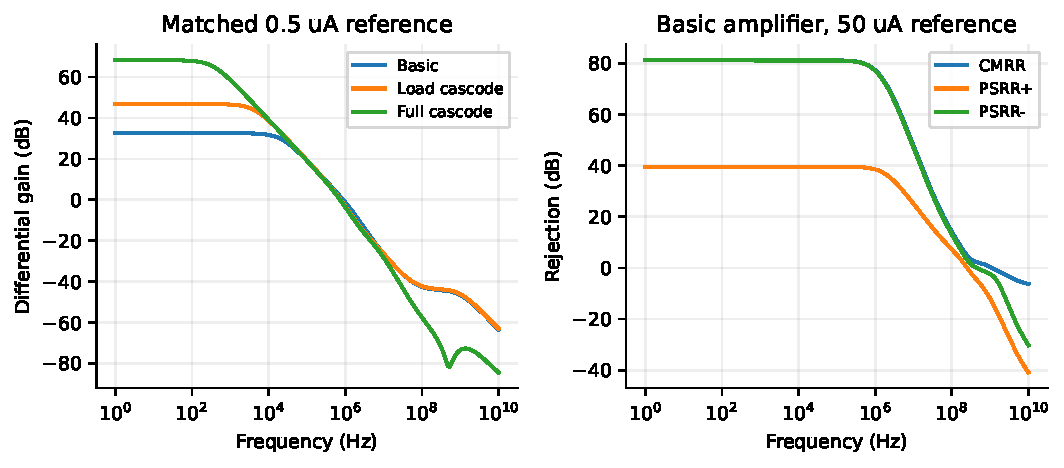
\includegraphics[width=\linewidth]{figures/voltage_amplifiers.pdf}
\caption{左：相同 0.5 微安參考的三種拓樸。右：50 微安基本型的拒斥比。兩圖的偏流不同。}
\end{figure}
三種拓樸在共同 0.5 $\mu$A 參考的掃描中，所有元件滿足 $|V_{DS}|\ge |V_{DSAT}|$ 的連續樣點區間分別為基本型 0.20--1.00 V、負載 cascode 0.20--0.95 V、全 cascode 0.20--0.55 V。端點只有 50 mV 解析度，且基本型上界碰到掃描邊界，不能宣稱邊界外仍有效。此判準也不代表強反轉或固定跨導。
\begin{center}\small\begin{tabular}{lrrrrr}\toprule
Case/Type & $|A_i|$ & $R_{in}$ (k$\Omega$) & $R_o$ (k$\Omega$) & $f_{3dB}$ (MHz) & $V_o$ (V) \\ \midrule
C0/s & 0.501 & 4.061 & -- & 112.679 & 0.013 \\
C0/c & 0.503 & 9.127 & -- & 340.870 & 0.014 \\
C0/d & 0.731 & 7.958 & -- & 49.273 & 0.013 \\
C1/s & 1.916 & 4.061 & 15.814 & 0.778 & 0.512 \\
C1/c & 1.864 & 9.133 & 16.392 & 0.792 & 0.514 \\
C1/d & 2.797 & 7.958 & 15.814 & 0.794 & 0.512 \\
C2/s & 18.415 & 4.059 & 9.522 & 0.459 & 0.502 \\
C2/c & 18.271 & 9.134 & 12.146 & 0.443 & 0.515 \\
C2/d & 158.918 & 36.990 & 9.525 & 0.440 & 0.502 \\
C3/s & 127.907 & 4.009 & 1.744 & 0.025 & 0.436 \\
C3/c & 150.941 & 9.135 & 3.316 & 0.022 & 0.534 \\
C3/d & 1511.730 & 121.390 & 0.271 & 0.022 & 0.082 \\
C13/s & 0.751 & 2.114 & -- & 0.302 & 0.921 \\
C13/c & 0.678 & 4.770 & -- & 0.319 & 0.923 \\
C13/d & 0.007 & 4.192 & -- & 290.717 & 0.533 \\
\bottomrule\end{tabular}\end{center}
\begin{center}\small\begin{tabular}{lrrrr}\toprule
Lower width ($\mu$m) & $|A_i|$ & $R_{in}$ (k$\Omega$) & $R_o$ (k$\Omega$) & $f_{3dB}$ (MHz) \\ \midrule
100 & 0.935 & 8.949 & 16.337 & 0.810 \\
1000 & 0.936 & 8.528 & 16.337 & 0.793 \\
10000 & 0.895 & 7.674 & 16.325 & 0.533 \\
\bottomrule\end{tabular}\end{center}

\begin{figure}[htbp]\centering
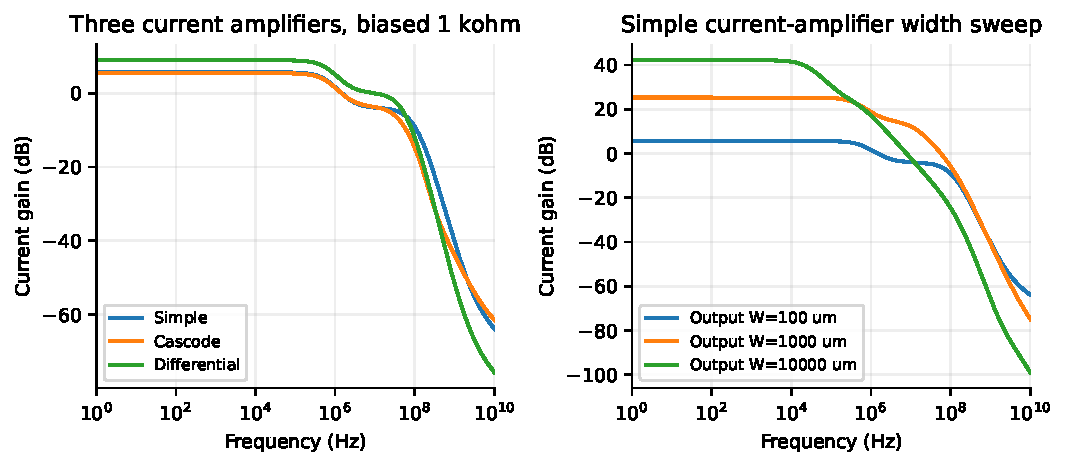
\includegraphics[width=\linewidth]{figures/current_amplifiers.pdf}
\caption{左：C1 的三種電流放大器。右：簡單型的輸出寬度掃描，包含實際偏壓與負載效應。}
\end{figure}
表內 s/c/d 分別為簡單／cascode／差動電流型。C0 的失效工作區、C13 的不平衡與所有實際電壓均保留；未把不符合平方律的結果刪除。未獨立量測的 Rout 標 --。圖與完整 CSV 包含更多頻率點，沒有把低頻增益當作全頻段增益。

\section{討論}
相較單端 CS，差動輸入可抑制共同擾動，容易接負回授，但增加元件、偏流、匹配需求及共模限制。等 W/L 拉長元件可降低輸出導納、提高增益；本次基本型由 39.60 dB 增至 45.44/46.53 dB，但頻寬降低。Cascode 提高輸出阻抗與增益，卻消耗電壓裕量；共同低電流下完整 cascode 的 ICMR 最窄。拒斥比均來自理想名義匹配，沒有失配或矽晶量測保證。

簡單電流鏡所需裕量與電容較小；cascode 的額外節點與 body effect 提高輸入阻抗，也可能降低負載電流增益。提高輸出 W 與偏流可提高理想鏡像倍率，但也提高電容及輸出導納，因此 Rin、Rout、GB 不會全部改善。PMOS 寬度改變時，DC 平衡也變；C13 的偏壓接近上軌，必須一起解讀。差動電流型可處理兩輸入之差，但本例有兩段鏡像，誤差與電容累積。PDF 46--47 的曲線文字、寬度表與圖名並不完全一致；本報告以明列的元件與案例辨識結果，不將舊數字當作必達值。

\section{結論}
Lab 4.A/B 所有拓樸、量測與討論均有對應。增益提升、拒斥與工作區的取捨有實際結果，失效偏壓亦保留；未宣稱原製程的數值或製造驗證已重現。

